\section{UML Export}

The \emph{reprotool.uml.export} plugin is responsible for exporting a \emph{reprotool} project into UML. A \emph{reprotool} user has
a possibility to create either a \emph{UML class diagram} or a \emph{UML use case diagram}. The UML model we use in \emph{reprotool}
comes from the \emph{org.eclipse.uml2.uml} eclipse plugin. This model is based on the EMF framework.

\subsection{UML class diagram}
The \emph{UML class diagram} contains class entities for every project actor and one class entity representing the \emph{system}.
The actors in the diagram are provided with activities that they perform.

\begin{figure}[ht]
  \centering
  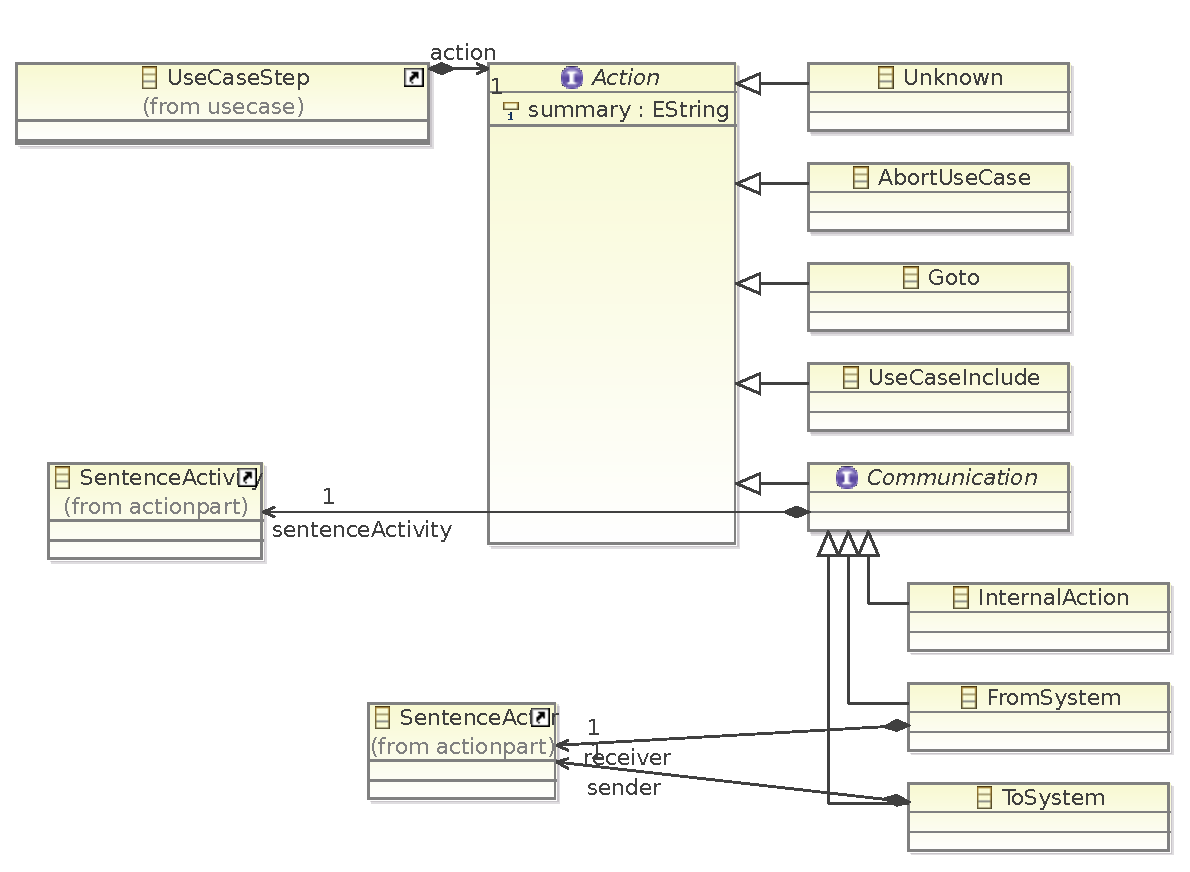
\includegraphics[width=\textwidth]{images/ReprotoolActionsModelSimple}
  \caption{Model of use-case step actions}
  \label{fig:ReprotoolActionsModel}
\end{figure}

Every use-case step can specify an activity for some
actor. This is achieved by assigning an \emph{action} of the type \emph{Communication} to the use-case step. The \emph{Communication}
actions can be either \emph{InternalAction}, \emph{FromSystem}, or \emph{ToSystem}. If the action is of type \emph{InternalAction},
or \emph{ToSystem}, the associated activity is performed on the actor representing the \emph{system}. Otherwise, if the action is of
type \emph{FromSystem}, the \emph{receiver} of the action determins the actor associated with the activity.

The UML class diagram model is generated in the \emph{UMLGen.xtend} class in the \emph{reprotool.uml.export.mapping} package of the
\emph{reprotool.uml.export} plugin. This whole process is simply a transformation of our use-case model into the UML class diagram
model. We utilised \emph{XTend} for this process to take advantage of some of its functional programming language features.

\subsection{UML use-case diagram}
The \emph{UML use-case diagram} contains actor entities for every project actor and use-case entities for every project use-case.
For every project use-case \emph{U} that has its \emph{primary actor} set, the diagram also contains a link between the use-case \emph{U}
and its primary actor. The diagram also depicts the \emph{include} relation between project use-cases. An \emph{include} relation between
two use-cases \emph{U1} and \emph{U2} will appear in the diagram, if there exists at least one execution path in use-case \emph{U1}
that contains a use-case step that includes use-case \emph{U2}.

The UML use-case diagram model is generated in the \emph{UMLUseCaseModelGenerator.xtend} class in the \emph{reprotool.uml.export.mapping} package of the
\emph{reprotool.uml.export} plugin. The whole process is a simple two-phase model transformation process. In the first phase, the
information about project actors and their associated use-cases is collected. In the second phase, the use-case include relations are
searched.

